\documentclass[11pt, oneside]{article}   	
\usepackage{geometry}                		
\geometry{letterpaper}                   		
\usepackage[parfill]{parskip}    		
\usepackage{graphicx}

%those two lines are needed to import the package			
\usepackage{tikz}
\usetikzlibrary{arrows}

\title{Brief Article}
\author{The Author}

\begin{document}
\maketitle

\section{problem 0}
\subsection{demonstration of how to draw a graph}

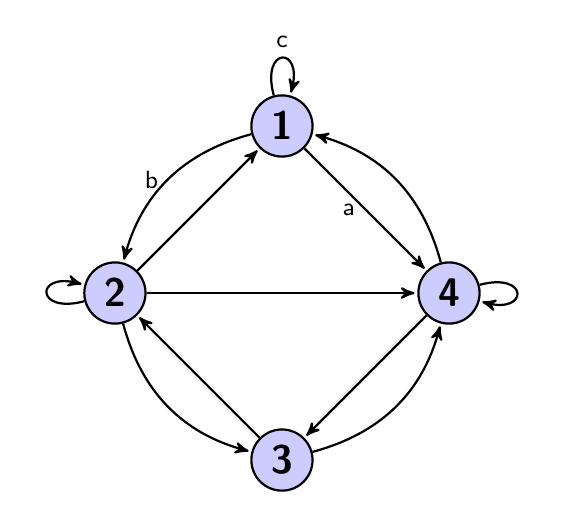
\begin{tikzpicture}[->,>=stealth',shorten >=1pt,auto,node distance=3cm,
  thick,main node/.style={circle,fill=blue!20,draw,font=\sffamily\Large\bfseries}]

  \node[main node] (1) {1}; 
  % the syntax of a node is: the id of this node, the alinement of this node, the label of this node
  \node[main node] (2) [below left of=1] {2};
  \node[main node] (3) [below right of=2] {3};
  \node[main node] (4) [below right of=1] {4};

  \path[every node/.style={font=\sffamily\small}]
    (1)	edge node [left] {a} (4)
        	edge [bend right] node[left] {b} (2)
        	edge [loop above] node {c} (1)
    (2)	edge node [right] {} (1)
        	edge node {} (4)
        	edge [loop left] node {} (2)
        	edge [bend right] node[left] {} (3)
    (3)	edge node [right] {} (2)
        	edge [bend right] node[right] {} (4)
    (4)	edge node [left] {} (3)
        	edge [loop right] node {} (4)
        	edge [bend right] node[right] {} (1);
\end{tikzpicture}

%problem 1
\section{Problem1}


%node like before union
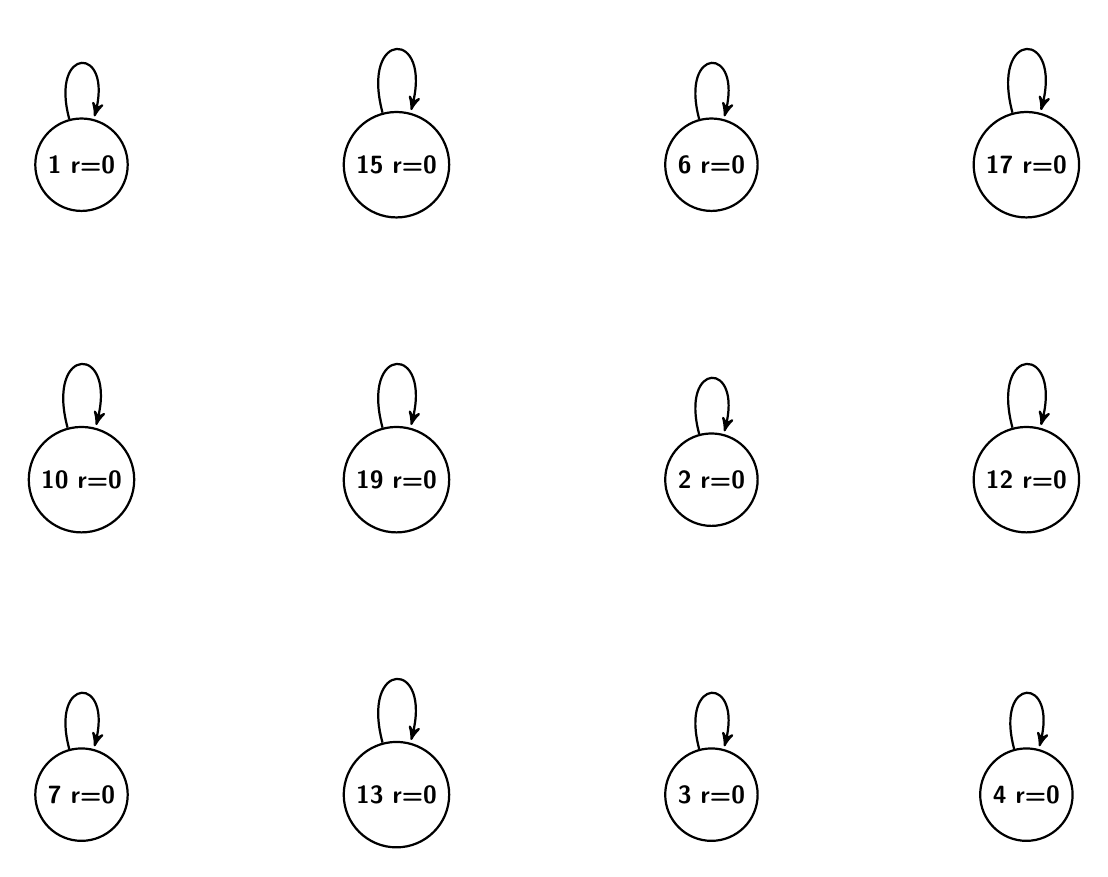
\begin{tikzpicture}[->,>=stealth',shorten >=1pt,auto,node distance=4cm,
  thick,main node/.style={circle,fill=white!20,draw,font=\sffamily\small\bfseries}]

 \node[main node] (1) {1 r=0}; 
 \node[main node] (15) [right of=1] {15 r=0}; 
 \node[main node] (6) [right of=15]  {6 r=0}; 
 \node[main node] (17) [right of=6]  {17 r=0}; 
 \node[main node] (10) [below of=1]  {10 r=0}; 
 \node[main node] (19) [right of=10]  {19 r=0}; 
 \node[main node] (2) [right of=19]  {2 r=0}; 
 \node[main node] (12) [right of=2]  {12 r=0}; 
 \node[main node] (7) [below of=10]  {7 r=0}; 
 \node[main node] (13) [right of=7] {13 r=0}; 
 \node[main node] (3) [right of=13]  {3 r=0}; 
 \node[main node] (4) [right of=3]  {4 r=0}; 


 \path[every node/.style={font=\sffamily\small}]
    (1)		edge [loop above] node {} (1)
    (2)		edge [loop above] node {} (2)
    (3)		edge [loop above] node {} (3)
    (4)		edge [loop above] node {} (4)
    (6)		edge [loop above] node {} (6)
    (7)		edge [loop above] node {} (7)
    (10)	edge [loop above] node {} (10)
    (12)	edge [loop above] node {} (12)
    (13)	 edge [loop above] node {} (13)
    (15)	 edge [loop above] node {} (15)
    (17)	 edge [loop above] node {} (17)
    (19)	 edge [loop above] node {} (19);
	
\end{tikzpicture}


%node like after union 1 15
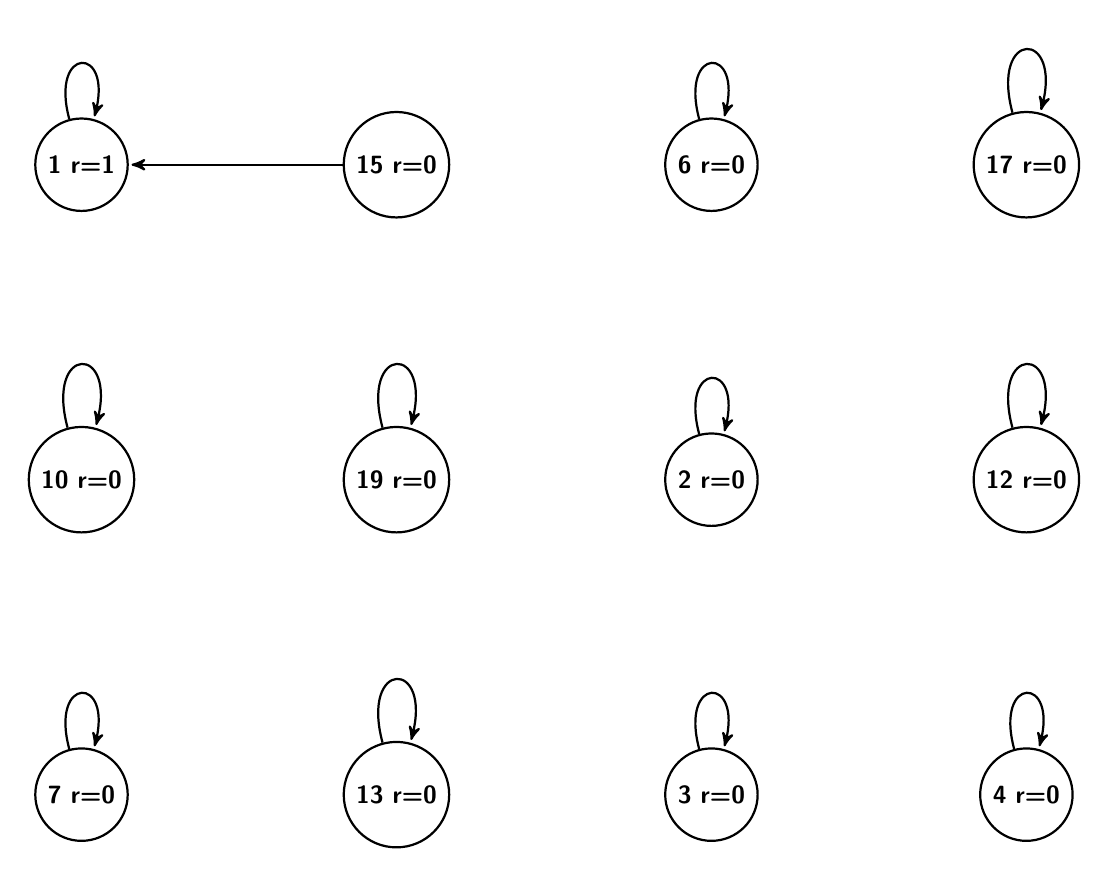
\begin{tikzpicture}[->,>=stealth',shorten >=1pt,auto,node distance=4cm,
  thick,main node/.style={circle,fill=white!20,draw,font=\sffamily\small\bfseries}]

 \node[main node] (1) {1 r=1}; 
 \node[main node] (15) [right of=1] {15 r=0}; 
 \node[main node] (6) [right of=15]  {6 r=0}; 
 \node[main node] (17) [right of=6]  {17 r=0}; 
 \node[main node] (10) [below of=1]  {10 r=0}; 
 \node[main node] (19) [right of=10]  {19 r=0}; 
 \node[main node] (2) [right of=19]  {2 r=0}; 
 \node[main node] (12) [right of=2]  {12 r=0}; 
 \node[main node] (7) [below of=10]  {7 r=0}; 
 \node[main node] (13) [right of=7] {13 r=0}; 
 \node[main node] (3) [right of=13]  {3 r=0}; 
 \node[main node] (4) [right of=3]  {4 r=0}; 


 \path[every node/.style={font=\sffamily\small}]
    (1)		edge [loop above] node {} (1)
    (2)		edge [loop above] node {} (2)
    (3)		edge [loop above] node {} (3)
    (4)		edge [loop above] node {} (4)
    (6)		edge [loop above] node {} (6)
    (7)		edge [loop above] node {} (7)
    (10)	edge [loop above] node {} (10)
    (12)	edge [loop above] node {} (12)
    (13)	 edge [loop above] node {} (13)
    (15)	 edge [left] node {} (1)
    (17)	 edge [loop above] node {} (17)
    (19)	 edge [loop above] node {} (19);
	
\end{tikzpicture}

%node like after union 6 17
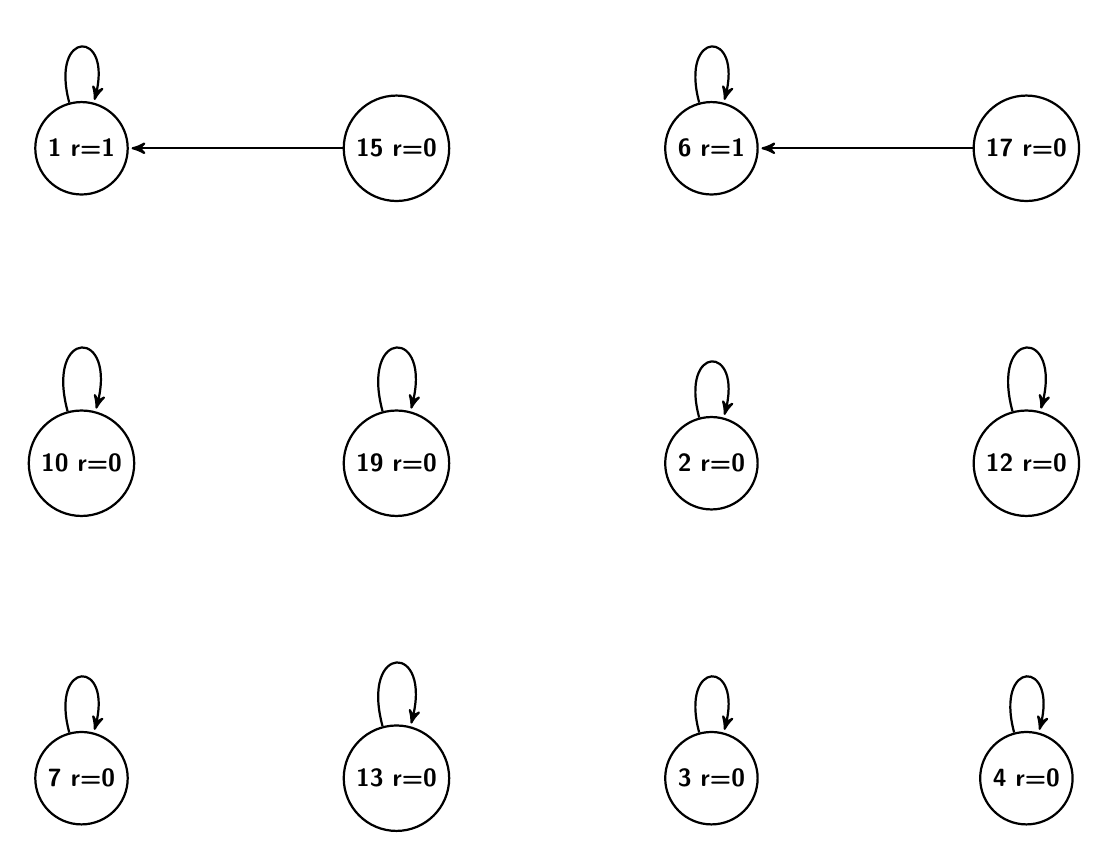
\begin{tikzpicture}[->,>=stealth',shorten >=1pt,auto,node distance=4cm,
  thick,main node/.style={circle,fill=white!20,draw,font=\sffamily\small\bfseries}]

 \node[main node] (1) {1 r=1}; 
 \node[main node] (15) [right of=1] {15 r=0}; 
 \node[main node] (6) [right of=15]  {6 r=1}; 
 \node[main node] (17) [right of=6]  {17 r=0}; 
 \node[main node] (10) [below of=1]  {10 r=0}; 
 \node[main node] (19) [right of=10]  {19 r=0}; 
 \node[main node] (2) [right of=19]  {2 r=0}; 
 \node[main node] (12) [right of=2]  {12 r=0}; 
 \node[main node] (7) [below of=10]  {7 r=0}; 
 \node[main node] (13) [right of=7] {13 r=0}; 
 \node[main node] (3) [right of=13]  {3 r=0}; 
 \node[main node] (4) [right of=3]  {4 r=0}; 


 \path[every node/.style={font=\sffamily\small}]
    (1)		edge [loop above] node {} (1)
    (2)		edge [loop above] node {} (2)
    (3)		edge [loop above] node {} (3)
    (4)		edge [loop above] node {} (4)
    (6)		edge [loop above] node {} (6)
    (7)		edge [loop above] node {} (7)
    (10)	edge [loop above] node {} (10)
    (12)	edge [loop above] node {} (12)
    (13)	 edge [loop above] node {} (13)
    (15)	 edge [left] node {} (1)
    (17)	 edge [left] node {} (6)
    (19)	 edge [loop above] node {} (19);
	
\end{tikzpicture}

%node like after union 10 19
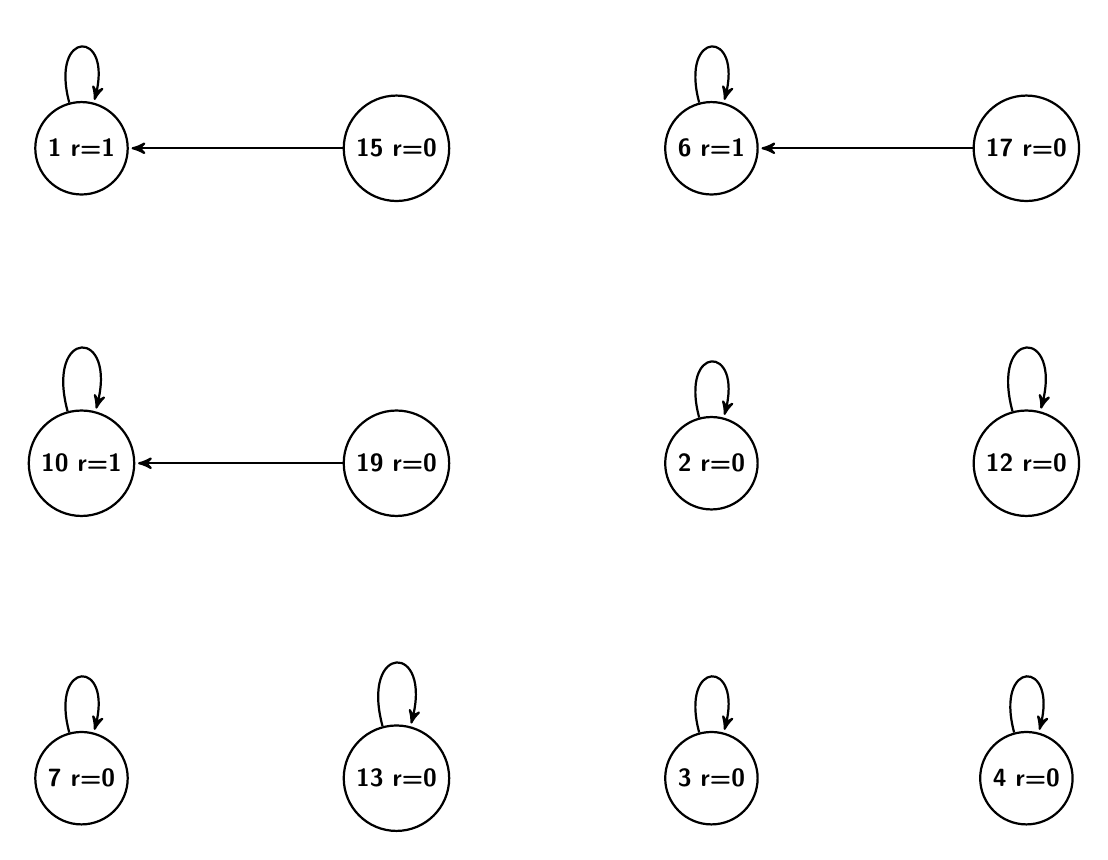
\begin{tikzpicture}[->,>=stealth',shorten >=1pt,auto,node distance=4cm,
  thick,main node/.style={circle,fill=white!20,draw,font=\sffamily\small\bfseries}]

 \node[main node] (1) {1 r=1}; 
 \node[main node] (15) [right of=1] {15 r=0}; 
 \node[main node] (6) [right of=15]  {6 r=1}; 
 \node[main node] (17) [right of=6]  {17 r=0}; 
 \node[main node] (10) [below of=1]  {10 r=1}; 
 \node[main node] (19) [right of=10]  {19 r=0}; 
 \node[main node] (2) [right of=19]  {2 r=0}; 
 \node[main node] (12) [right of=2]  {12 r=0}; 
 \node[main node] (7) [below of=10]  {7 r=0}; 
 \node[main node] (13) [right of=7] {13 r=0}; 
 \node[main node] (3) [right of=13]  {3 r=0}; 
 \node[main node] (4) [right of=3]  {4 r=0}; 


 \path[every node/.style={font=\sffamily\small}]
    (1)		edge [loop above] node {} (1)
    (2)		edge [loop above] node {} (2)
    (3)		edge [loop above] node {} (3)
    (4)		edge [loop above] node {} (4)
    (6)		edge [loop above] node {} (6)
    (7)		edge [loop above] node {} (7)
    (10)	edge [loop above] node {} (10)
    (12)	edge [loop above] node {} (12)
    (13)	 edge [loop above] node {} (13)
    (15)	 edge [left] node {} (1)
    (17)	 edge [left] node {} (6)
    (19)	 edge [left] node {} (10);
	
\end{tikzpicture}


%node like after union 1 2
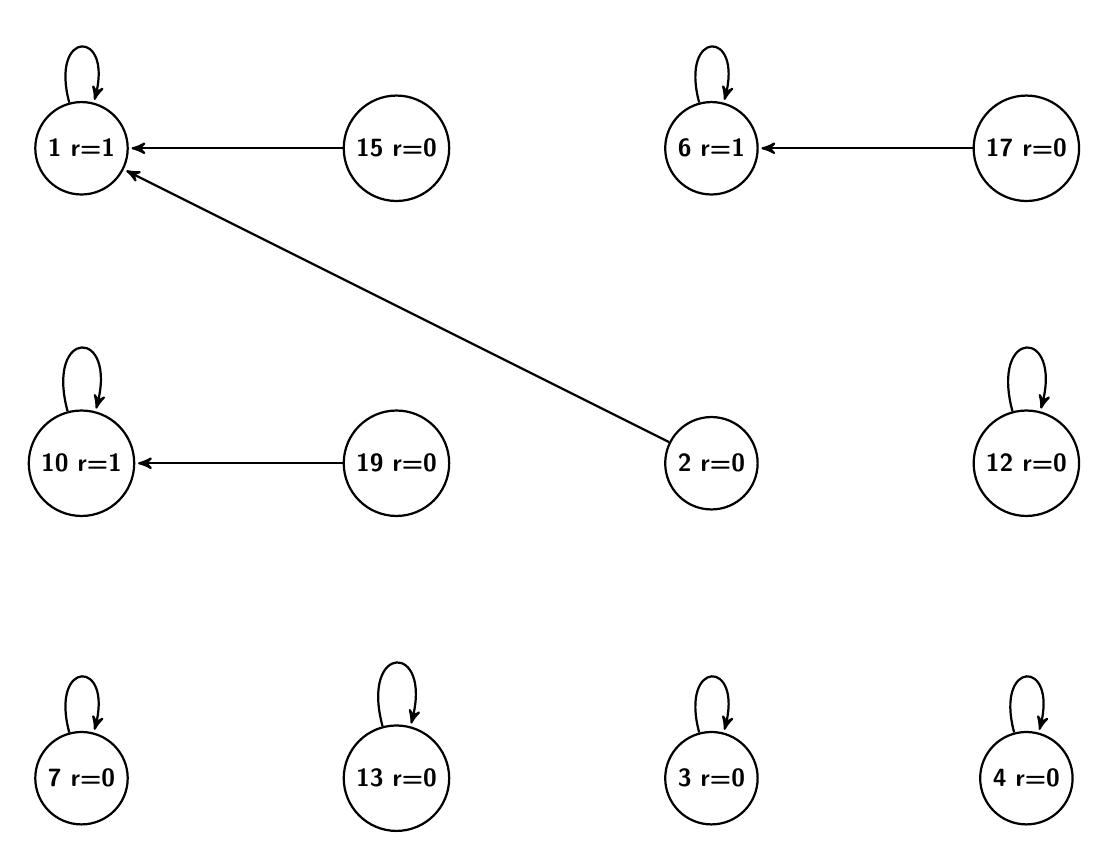
\begin{tikzpicture}[->,>=stealth',shorten >=1pt,auto,node distance=4cm,
  thick,main node/.style={circle,fill=white!20,draw,font=\sffamily\small\bfseries}]

 \node[main node] (1) {1 r=1}; 
 \node[main node] (15) [right of=1] {15 r=0}; 
 \node[main node] (6) [right of=15]  {6 r=1}; 
 \node[main node] (17) [right of=6]  {17 r=0}; 
 \node[main node] (10) [below of=1]  {10 r=1}; 
 \node[main node] (19) [right of=10]  {19 r=0}; 
 \node[main node] (2) [right of=19]  {2 r=0}; 
 \node[main node] (12) [right of=2]  {12 r=0}; 
 \node[main node] (7) [below of=10]  {7 r=0}; 
 \node[main node] (13) [right of=7] {13 r=0}; 
 \node[main node] (3) [right of=13]  {3 r=0}; 
 \node[main node] (4) [right of=3]  {4 r=0}; 


 \path[every node/.style={font=\sffamily\small}]
    (1)		edge [loop above] node {} (1)
    (2)		edge [above] node {} (1)
    (3)		edge [loop above] node {} (3)
    (4)		edge [loop above] node {} (4)
    (6)		edge [loop above] node {} (6)
    (7)		edge [loop above] node {} (7)
    (10)	edge [loop above] node {} (10)
    (12)	edge [loop above] node {} (12)
    (13)	 edge [loop above] node {} (13)
    (15)	 edge [left] node {} (1)
    (17)	 edge [left] node {} (6)
    (19)	 edge [left] node {} (10);
	
\end{tikzpicture}

%node like after union 2 12
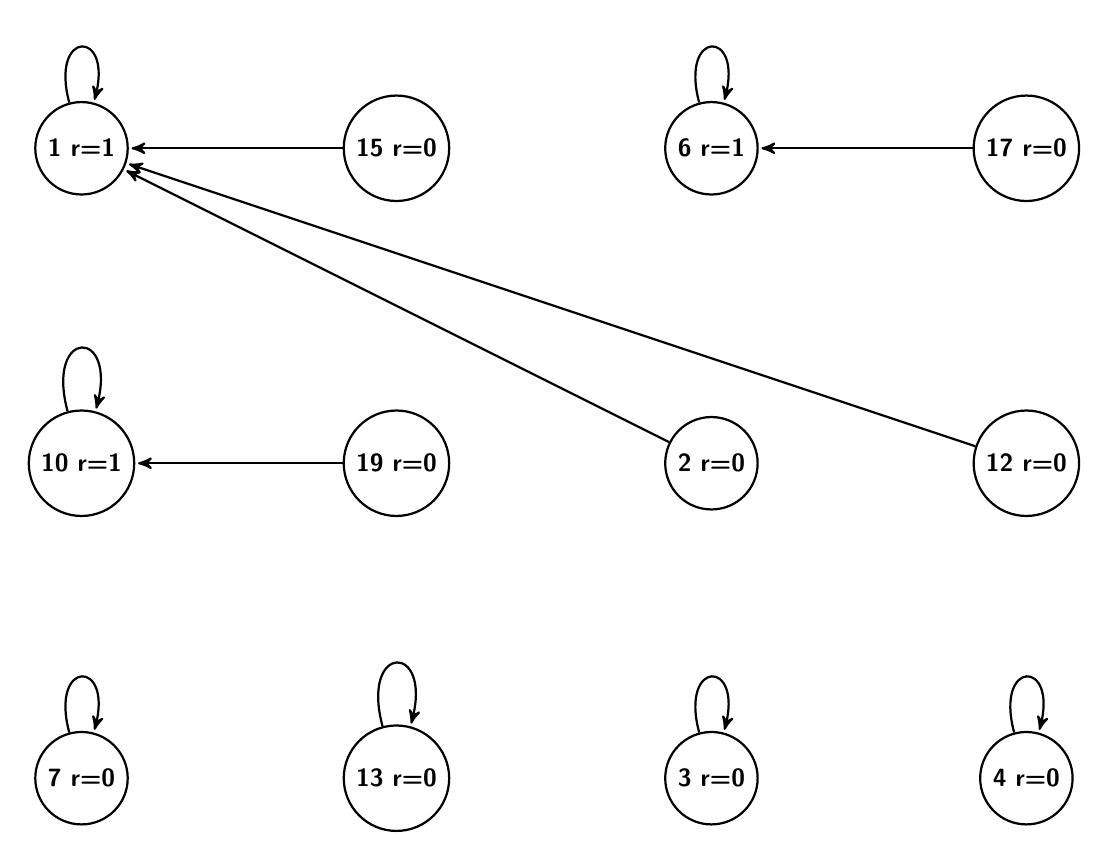
\begin{tikzpicture}[->,>=stealth',shorten >=1pt,auto,node distance=4cm,
  thick,main node/.style={circle,fill=white!20,draw,font=\sffamily\small\bfseries}]

 \node[main node] (1) {1 r=1}; 
 \node[main node] (15) [right of=1] {15 r=0}; 
 \node[main node] (6) [right of=15]  {6 r=1}; 
 \node[main node] (17) [right of=6]  {17 r=0}; 
 \node[main node] (10) [below of=1]  {10 r=1}; 
 \node[main node] (19) [right of=10]  {19 r=0}; 
 \node[main node] (2) [right of=19]  {2 r=0}; 
 \node[main node] (12) [right of=2]  {12 r=0}; 
 \node[main node] (7) [below of=10]  {7 r=0}; 
 \node[main node] (13) [right of=7] {13 r=0}; 
 \node[main node] (3) [right of=13]  {3 r=0}; 
 \node[main node] (4) [right of=3]  {4 r=0}; 


 \path[every node/.style={font=\sffamily\small}]
    (1)		edge [loop above] node {} (1)
    (2)		edge [above] node {} (1)
    (3)		edge [loop above] node {} (3)
    (4)		edge [loop above] node {} (4)
    (6)		edge [loop above] node {} (6)
    (7)		edge [loop above] node {} (7)
    (10)	edge [loop above] node {} (10)
    (12)	edge [above] node {} (1)
    (13)	 edge [loop above] node {} (13)
    (15)	 edge [left] node {} (1)
    (17)	 edge [left] node {} (6)
    (19)	 edge [left] node {} (10);
	
\end{tikzpicture}

%node like after union 17 15
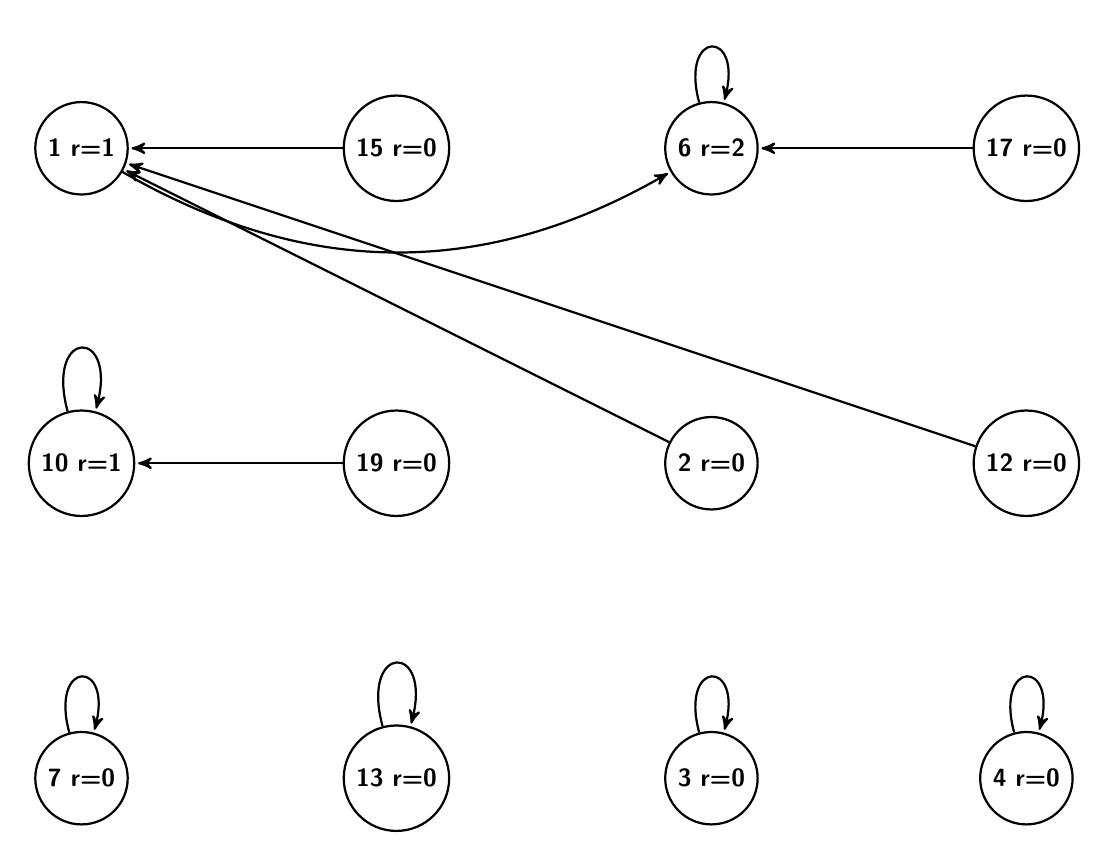
\begin{tikzpicture}[->,>=stealth',shorten >=1pt,auto,node distance=4cm,
  thick,main node/.style={circle,fill=white!20,draw,font=\sffamily\small\bfseries}]

 \node[main node] (1) {1 r=1}; 
 \node[main node] (15) [right of=1] {15 r=0}; 
 \node[main node] (6) [right of=15]  {6 r=2}; 
 \node[main node] (17) [right of=6]  {17 r=0}; 
 \node[main node] (10) [below of=1]  {10 r=1}; 
 \node[main node] (19) [right of=10]  {19 r=0}; 
 \node[main node] (2) [right of=19]  {2 r=0}; 
 \node[main node] (12) [right of=2]  {12 r=0}; 
 \node[main node] (7) [below of=10]  {7 r=0}; 
 \node[main node] (13) [right of=7] {13 r=0}; 
 \node[main node] (3) [right of=13]  {3 r=0}; 
 \node[main node] (4) [right of=3]  {4 r=0}; 


 \path[every node/.style={font=\sffamily\small}]
    (1)		edge [bend right] node[left] {} (6)
    (2)		edge [above] node {} (1)
    (3)		edge [loop above] node {} (3)
    (4)		edge [loop above] node {} (4)
    (6)		edge [loop above] node {} (6)
    (7)		edge [loop above] node {} (7)
    (10)	edge [loop above] node {} (10)
    (12)	edge [above] node {} (1)
    (13)	 edge [loop above] node {} (13)
    (15)	 edge [left] node {} (1)
    (17)	 edge [left] node {} (6)
    (19)	 edge [left] node {} (10);
	
\end{tikzpicture}

%node like after union 7 13
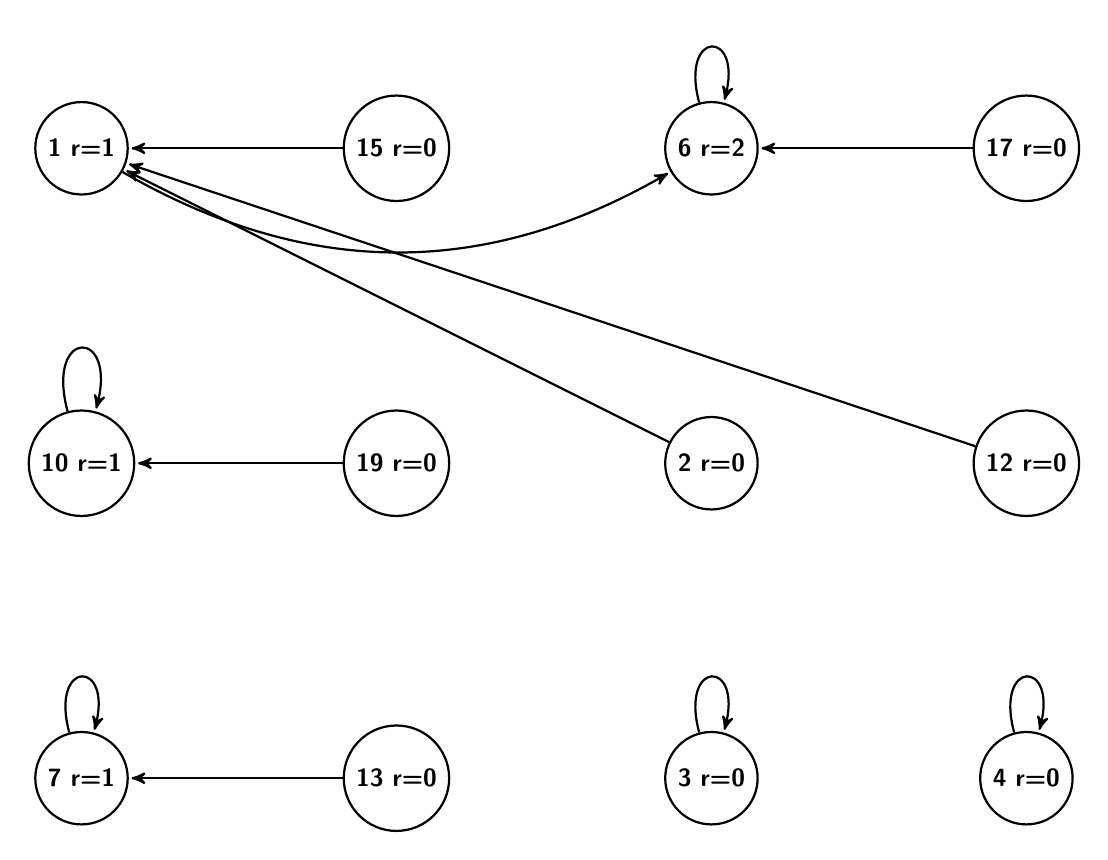
\begin{tikzpicture}[->,>=stealth',shorten >=1pt,auto,node distance=4cm,
  thick,main node/.style={circle,fill=white!20,draw,font=\sffamily\small\bfseries}]

 \node[main node] (1) {1 r=1}; 
 \node[main node] (15) [right of=1] {15 r=0}; 
 \node[main node] (6) [right of=15]  {6 r=2}; 
 \node[main node] (17) [right of=6]  {17 r=0}; 
 \node[main node] (10) [below of=1]  {10 r=1}; 
 \node[main node] (19) [right of=10]  {19 r=0}; 
 \node[main node] (2) [right of=19]  {2 r=0}; 
 \node[main node] (12) [right of=2]  {12 r=0}; 
 \node[main node] (7) [below of=10]  {7 r=1}; 
 \node[main node] (13) [right of=7] {13 r=0}; 
 \node[main node] (3) [right of=13]  {3 r=0}; 
 \node[main node] (4) [right of=3]  {4 r=0}; 


 \path[every node/.style={font=\sffamily\small}]
    (1)		edge [bend right] node[left] {} (6)
    (2)		edge [above] node {} (1)
    (3)		edge [loop above] node {} (3)
    (4)		edge [loop above] node {} (4)
    (6)		edge [loop above] node {} (6)
    (7)		edge [loop above] node {} (7)
    (10)	edge [loop above] node {} (10)
    (12)	edge [above] node {} (1)
    (13)	 edge [above] node {} (7)
    (15)	 edge [left] node {} (1)
    (17)	 edge [left] node {} (6)
    (19)	 edge [left] node {} (10);
	
\end{tikzpicture}

%node like after union 19 3
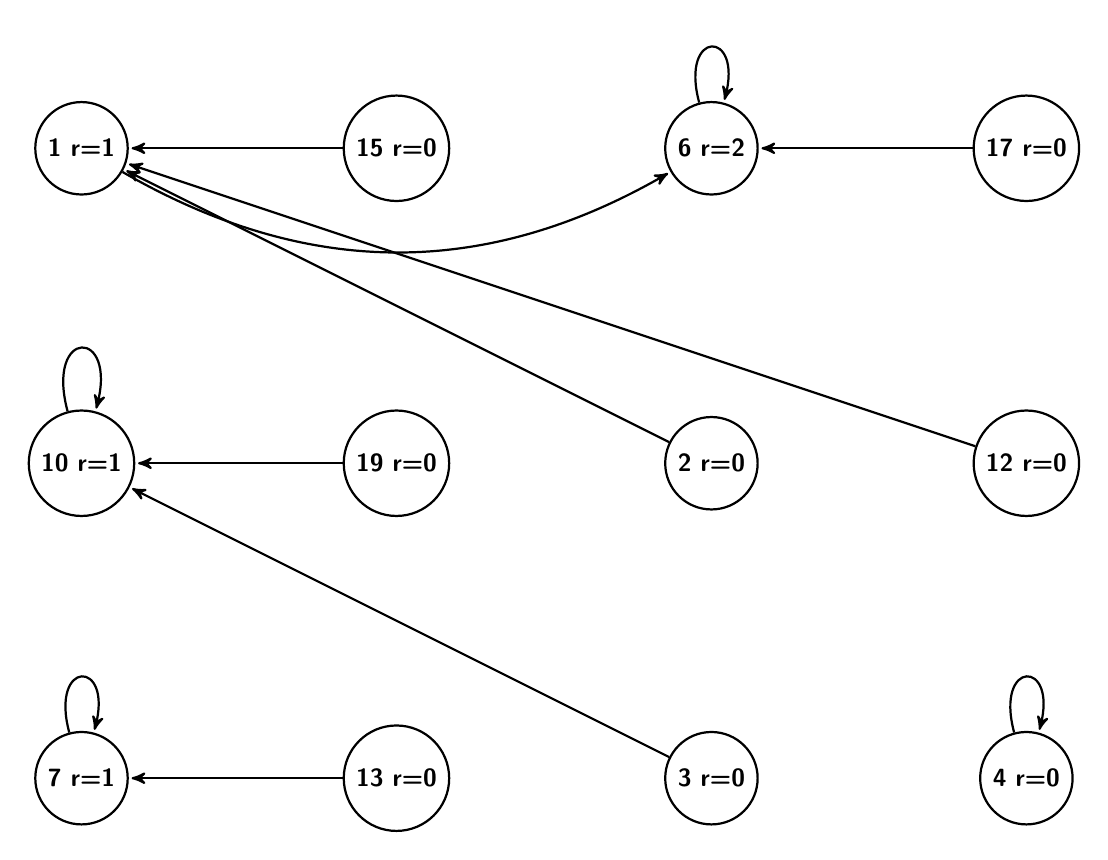
\begin{tikzpicture}[->,>=stealth',shorten >=1pt,auto,node distance=4cm,
  thick,main node/.style={circle,fill=white!20,draw,font=\sffamily\small\bfseries}]

 \node[main node] (1) {1 r=1}; 
 \node[main node] (15) [right of=1] {15 r=0}; 
 \node[main node] (6) [right of=15]  {6 r=2}; 
 \node[main node] (17) [right of=6]  {17 r=0}; 
 \node[main node] (10) [below of=1]  {10 r=1}; 
 \node[main node] (19) [right of=10]  {19 r=0}; 
 \node[main node] (2) [right of=19]  {2 r=0}; 
 \node[main node] (12) [right of=2]  {12 r=0}; 
 \node[main node] (7) [below of=10]  {7 r=1}; 
 \node[main node] (13) [right of=7] {13 r=0}; 
 \node[main node] (3) [right of=13]  {3 r=0}; 
 \node[main node] (4) [right of=3]  {4 r=0}; 


 \path[every node/.style={font=\sffamily\small}]
    (1)		edge [bend right] node[left] {} (6)
    (2)		edge [above] node {} (1)
    (3)		edge [above] node {} (10)
    (4)		edge [loop above] node {} (4)
    (6)		edge [loop above] node {} (6)
    (7)		edge [loop above] node {} (7)
    (10)	edge [loop above] node {} (10)
    (12)	edge [above] node {} (1)
    (13)	 edge [above] node {} (7)
    (15)	 edge [left] node {} (1)
    (17)	 edge [left] node {} (6)
    (19)	 edge [left] node {} (10);
	
\end{tikzpicture}


%node like after union 4 7
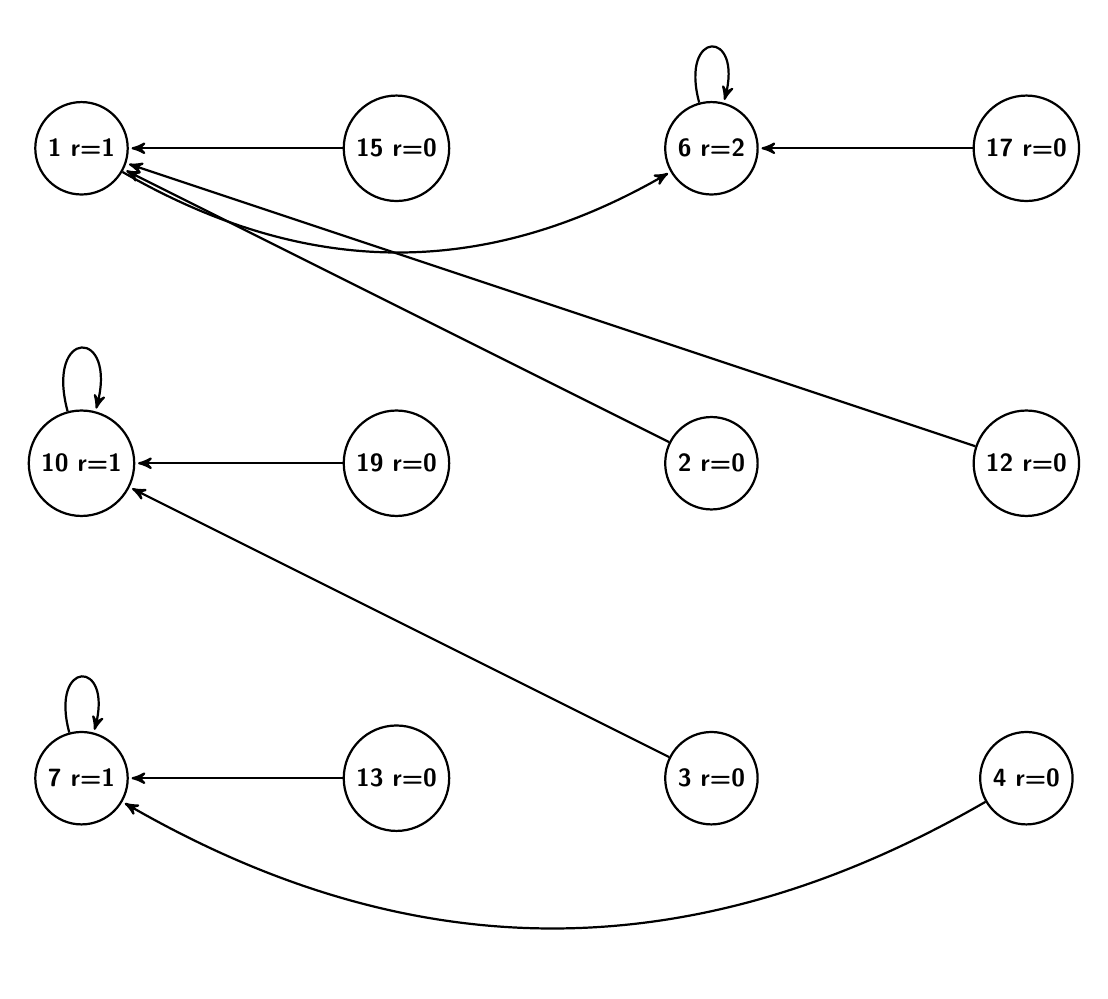
\begin{tikzpicture}[->,>=stealth',shorten >=1pt,auto,node distance=4cm,
  thick,main node/.style={circle,fill=white!20,draw,font=\sffamily\small\bfseries}]

 \node[main node] (1) {1 r=1}; 
 \node[main node] (15) [right of=1] {15 r=0}; 
 \node[main node] (6) [right of=15]  {6 r=2}; 
 \node[main node] (17) [right of=6]  {17 r=0}; 
 \node[main node] (10) [below of=1]  {10 r=1}; 
 \node[main node] (19) [right of=10]  {19 r=0}; 
 \node[main node] (2) [right of=19]  {2 r=0}; 
 \node[main node] (12) [right of=2]  {12 r=0}; 
 \node[main node] (7) [below of=10]  {7 r=1}; 
 \node[main node] (13) [right of=7] {13 r=0}; 
 \node[main node] (3) [right of=13]  {3 r=0}; 
 \node[main node] (4) [right of=3]  {4 r=0}; 


 \path[every node/.style={font=\sffamily\small}]
    (1)		edge [bend right] node[left] {} (6)
    (2)		edge [above] node {} (1)
    (3)		edge [above] node {} (10)
    (4)		edge [bend left] node {} (7)
    (6)		edge [loop above] node {} (6)
    (7)		edge [loop above] node {} (7)
    (10)	edge [loop above] node {} (10)
    (12)	edge [above] node {} (1)
    (13)	 edge [above] node {} (7)
    (15)	 edge [left] node {} (1)
    (17)	 edge [left] node {} (6)
    (19)	 edge [left] node {} (10);
	
\end{tikzpicture}

%node like after union 4 3
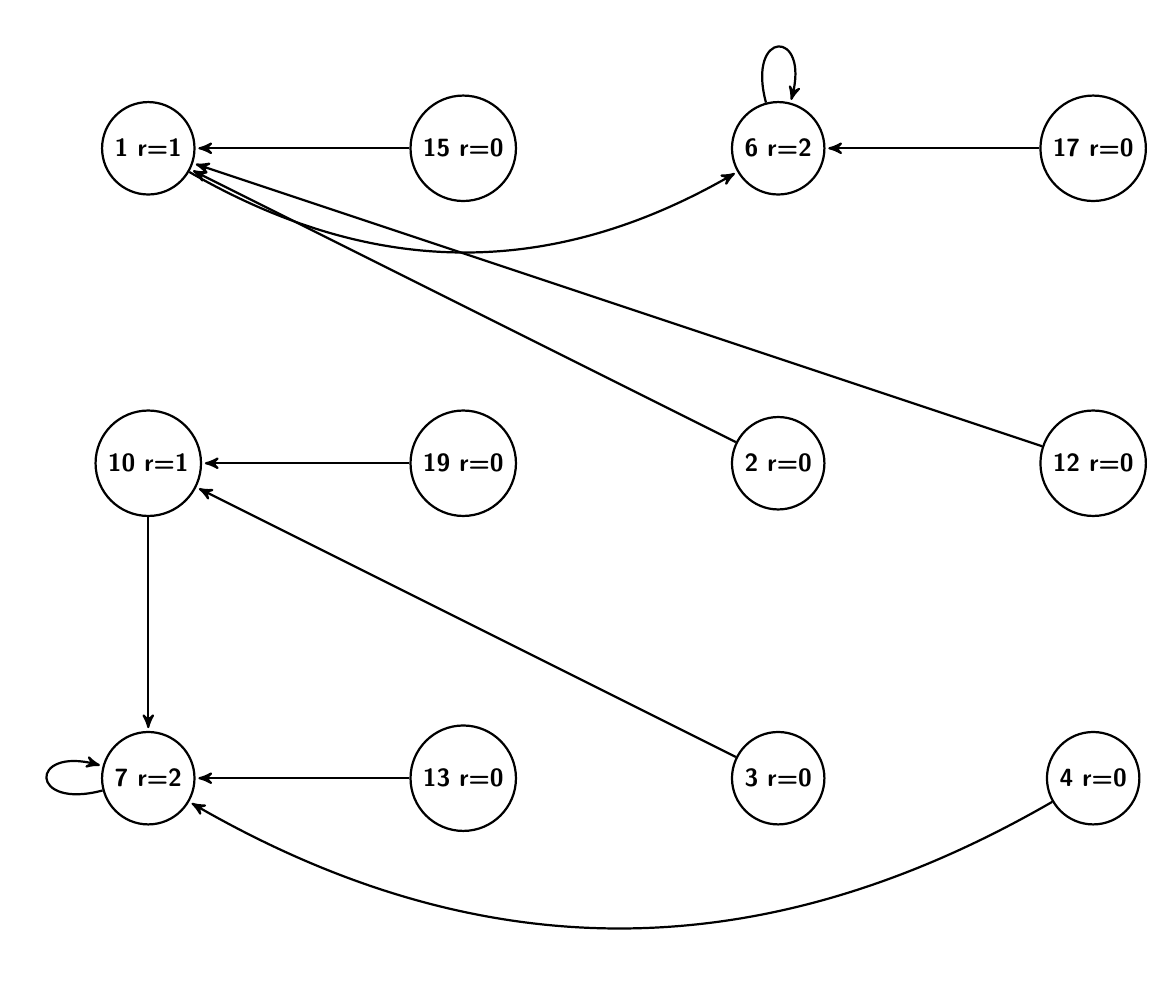
\begin{tikzpicture}[->,>=stealth',shorten >=1pt,auto,node distance=4cm,
  thick,main node/.style={circle,fill=white!20,draw,font=\sffamily\small\bfseries}]

 \node[main node] (1) {1 r=1}; 
 \node[main node] (15) [right of=1] {15 r=0}; 
 \node[main node] (6) [right of=15]  {6 r=2}; 
 \node[main node] (17) [right of=6]  {17 r=0}; 
 \node[main node] (10) [below of=1]  {10 r=1}; 
 \node[main node] (19) [right of=10]  {19 r=0}; 
 \node[main node] (2) [right of=19]  {2 r=0}; 
 \node[main node] (12) [right of=2]  {12 r=0}; 
 \node[main node] (7) [below of=10]  {7 r=2}; 
 \node[main node] (13) [right of=7] {13 r=0}; 
 \node[main node] (3) [right of=13]  {3 r=0}; 
 \node[main node] (4) [right of=3]  {4 r=0}; 


 \path[every node/.style={font=\sffamily\small}]
    (1)		edge [bend right] node[left] {} (6)
    (2)		edge [above] node {} (1)
    (3)		edge [above] node {} (10)
    (4)		edge [bend left] node {} (7)
    (6)		edge [loop above] node {} (6)
    (7)		edge [loop left] node {} (7)
    (10)	edge [below] node {} (7)
    (12)	edge [above] node {} (1)
    (13)	 edge [above] node {} (7)
    (15)	 edge [left] node {} (1)
    (17)	 edge [left] node {} (6)
    (19)	 edge [left] node {} (10);
	
\end{tikzpicture}

%node like after union 17 13
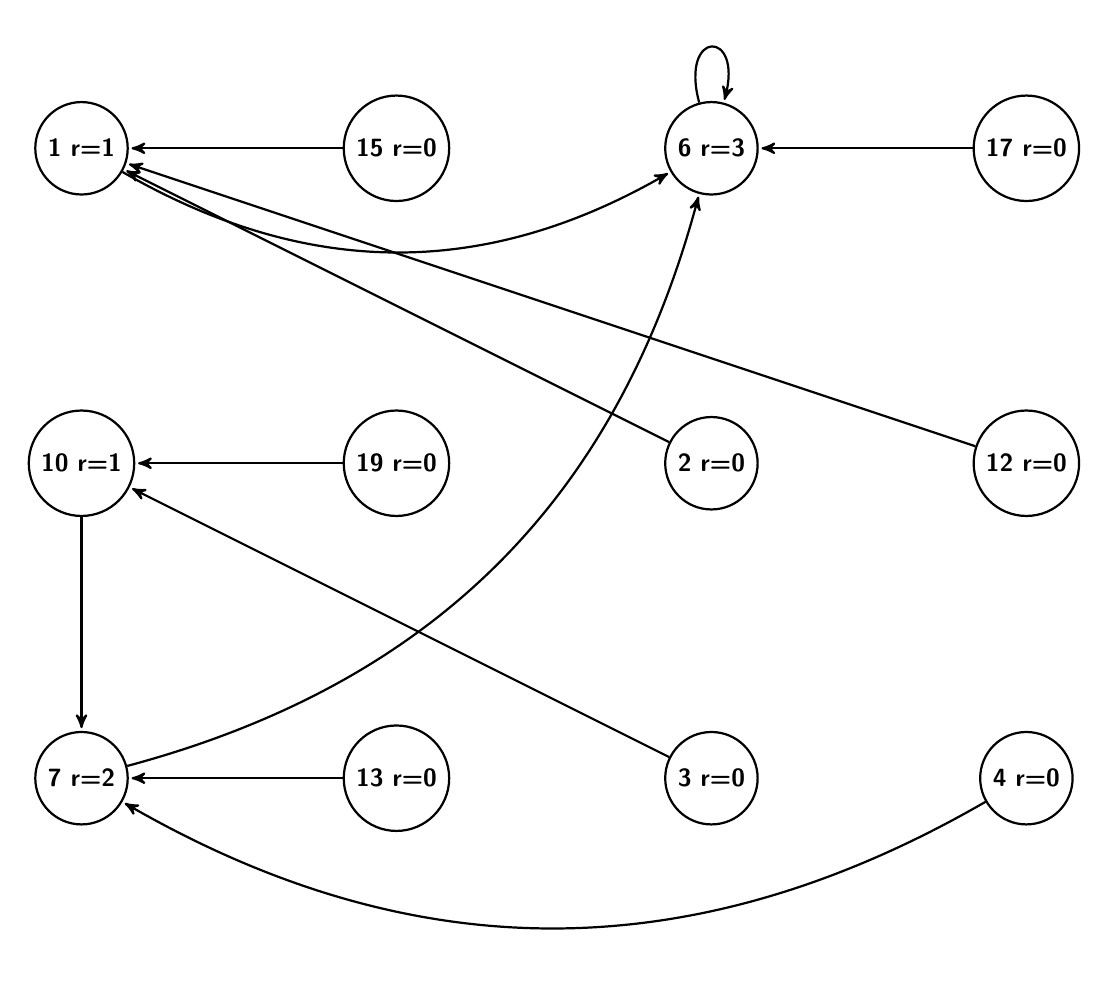
\begin{tikzpicture}[->,>=stealth',shorten >=1pt,auto,node distance=4cm,
  thick,main node/.style={circle,fill=white!20,draw,font=\sffamily\small\bfseries}]

 \node[main node] (1) {1 r=1}; 
 \node[main node] (15) [right of=1] {15 r=0}; 
 \node[main node] (6) [right of=15]  {6 r=3}; 
 \node[main node] (17) [right of=6]  {17 r=0}; 
 \node[main node] (10) [below of=1]  {10 r=1}; 
 \node[main node] (19) [right of=10]  {19 r=0}; 
 \node[main node] (2) [right of=19]  {2 r=0}; 
 \node[main node] (12) [right of=2]  {12 r=0}; 
 \node[main node] (7) [below of=10]  {7 r=2}; 
 \node[main node] (13) [right of=7] {13 r=0}; 
 \node[main node] (3) [right of=13]  {3 r=0}; 
 \node[main node] (4) [right of=3]  {4 r=0}; 


 \path[every node/.style={font=\sffamily\small}]
    (1)		edge [bend right] node[left] {} (6)
    (2)		edge [above] node {} (1)
    (3)		edge [above] node {} (10)
    (4)		edge [bend left] node {} (7)
    (6)		edge [loop above] node {} (6)
    (7)		edge [bend right] node {} (6)
    (10)	edge [below] node {} (7)
    (12)	edge [above] node {} (1)
    (13)	 edge [above] node {} (7)
    (15)	 edge [left] node {} (1)
    (17)	 edge [left] node {} (6)
    (19)	 edge [left] node {} (10);
	
\end{tikzpicture}


\end{document}  